% !TeX root = ../main.tex

% ----------------------------------------------------------
% Capítulo 2 (Integrante 2)
% ----------------------------------------------------------
\chapter[Busca Local e Estudo de Caso no TSP]{Busca Local e Estudo de Caso no TSP}

A Heurística do Vizinho Mais Próximo, apresentada no capítulo anterior, constrói uma rota viável em tempo polinomial, mas decide cada passo com base apenas na cidade atual. Essa visão local produz rotas que podem conter conexões longas ou cruzamentos, mesmo quando existe uma rota significativamente melhor. A busca local parte desse resultado e tenta corrigi-lo por meio de pequenas alterações na rota. Neste capítulo, apresentamos o conceito de busca local, o funcionamento das estratégias de melhoria, as principais operações de troca no TSP e um estudo de caso com cinco cidades, no qual comparamos a solução inicial com a solução obtida após as tentativas de melhoria.

\section{Conceito de Busca Local}

Considere um problema de otimização combinatória em que cada solução viável $s$ pertence a um conjunto finito $S$ e possui um custo $f(s)$. Para cada solução $s$, define-se uma vizinhança $N(s) \subseteq S$, formada pelas soluções que podem ser obtidas a partir de $s$ por um movimento elementar. A busca local é uma heurística iterativa que parte de uma solução inicial $s_0$ e, a cada passo, examina os vizinhos da solução corrente; se algum vizinho $s'$ tem custo menor, a busca se desloca para ele e o processo continua. Quando nenhum vizinho melhora o custo, a solução corrente é um ótimo local \cite{aarts2003, goldbarg2005}.

De modo mais preciso, um movimento é aceito quando
\begin{equation}
    f(s') < f(s), \quad s' \in N(s),
    \label{eq:aceitacao-busca-local}
\end{equation}
e a busca termina quando essa condição não vale para nenhum vizinho. Todo ótimo global é também ótimo local, pois nenhuma solução vizinha pode ter custo menor; a recíproca, porém, não é verdadeira. Uma solução pode ser a melhor de sua vizinhança e ainda assim estar distante da melhor solução global. O conjunto de soluções iniciais que convergem para um mesmo ótimo local é chamado de bacia de atração. Essa dependência da solução inicial e da definição de vizinhança é a razão pela qual a busca local não oferece garantia de otimalidade global \cite{russell2013}.

Há duas regras clássicas de escolha. Na melhor melhoria (\textit{best improvement}), todos os vizinhos são avaliados e escolhe-se o de menor custo. Na primeira melhoria (\textit{first improvement}), aceita-se o primeiro vizinho que reduza o custo, o que pode ser mais rápido quando a vizinhança é grande. Como o custo diminui estritamente e $S$ é finito, o processo termina em um número finito de iterações; entretanto, esse número não é limitado por um polinômio no tamanho da entrada, e o custo de cada iteração depende de $|N(s)|$ \cite{papadimitriou1977, englert2014}.

\section{Funcionamento de Estratégias de Melhoria de Soluções}

Uma estratégia de melhoria de soluções é definida por cinco elementos: a representação da solução, a função de custo, a vizinhança, o critério de aceitação e o critério de parada. A representação e a vizinhança determinam o alcance da busca; a função de custo orienta a escolha; o critério de aceitação define se um vizinho pode substituir a solução corrente; e o critério de parada interrompe o processo quando não há melhoria ou quando um limite de tempo é atingido \cite{goldbarg2005, souza_ufop}.

O Algoritmo~\ref{alg:busca-local} apresenta uma versão com a regra da melhor melhoria. Em cada iteração, toda a vizinhança é percorrida, o vizinho de menor custo é guardado e a solução corrente só é substituída se houver ganho. A variante de primeira melhoria substitui o laço interno por uma busca que interrompe assim que encontra o primeiro vizinho com custo menor, reiniciando a partir dele. Em ambos os casos, o algoritmo para quando nenhum movimento reduz o custo, o que caracteriza um ótimo local \cite{aarts2003}.

\begin{algorithm}[ht]
\caption{Busca local com regra da melhor melhoria.}
\label{alg:busca-local}
\begin{algorithmic}[1]
\STATE $s \gets s_0$
\WHILE{verdadeiro}
    \STATE $s_{\text{melhor}} \gets s$
    \FOR{cada $s' \in N(s)$}
        \IF{$f(s') < f(s_{\text{melhor}})$}
            \STATE $s_{\text{melhor}} \gets s'$
        \ENDIF
    \ENDFOR
    \IF{$f(s_{\text{melhor}}) \ge f(s)$}
        \RETURN $s$
    \ENDIF
    \STATE $s \gets s_{\text{melhor}}$
\ENDWHILE
\end{algorithmic}
\footnotesize{\textit{Fonte:} Elaborado pelos autores (2026)}
\end{algorithm}

A busca local pura pode ser combinada com mecanismos de diversificação. O multi-start executa a busca a partir de várias soluções iniciais e mantém a melhor. A busca local iterada (\textit{Iterated Local Search} -- ILS) perturba a solução corrente com um movimento de grande alcance e aplica novamente a busca local, aceitando a nova solução se ela for melhor. O tabu search mantém uma memória de movimentos recentes para evitar ciclos, e o simulated annealing aceita, com certa probabilidade, movimentos que pioram o custo, permitindo escapar de ótimos locais. Essas meta-heurísticas preservam a estrutura básica da busca local, mas trocam parte da simplicidade por maior capacidade de exploração \cite{souza_ufop, goldbarg2005, aarts2003}.

No TSP, a busca local é particularmente natural porque uma rota é uma permutação das cidades e qualquer alteração na ordem produz uma rota vizinha. A solução inicial pode ser obtida pela Heurística do Vizinho Mais Próximo, apresentada no capítulo anterior, ou por outra construção rápida. A busca local não substitui o algoritmo construtivo: ela o complementa, corrigindo decisões locais ruins que a construção gulosa não conseguiu prever. O custo por iteração depende do número de movimentos da vizinhança e do custo de avaliar cada movimento; para o 2-opt, por exemplo, há $O(n^2)$ movimentos por iteração \cite{croes1958, johnson1997}.

\section{Exemplos de Operações de Troca ou Reorganização de Rotas}

A operação mais conhecida é o 2-opt \cite{croes1958}. Seja uma rota $T = (t_1, \dots, t_n)$, com $t_{n+1} = t_1$. O movimento remove duas arestas não adjacentes, $\{t_i, t_{i+1}\}$ e $\{t_j, t_{j+1}\}$, e as substitui por $\{t_i, t_j\}$ e $\{t_{i+1}, t_{j+1}\}$. Para que o resultado continue sendo um ciclo, o trecho $t_{i+1}, \dots, t_j$ é invertido. A variação de custo é
\begin{equation}
    \Delta(i,j) = d(t_i,t_j) + d(t_{i+1},t_{j+1}) - d(t_i,t_{i+1}) - d(t_j,t_{j+1}),
    \label{eq:delta-2opt}
\end{equation}
e o movimento é aceito quando $\Delta(i,j) < 0$. O número de pares de arestas não adjacentes é $n(n-3)/2$, o que dá $O(n^2)$ movimentos por iteração; a inversão do trecho custa $O(n)$ \cite{croes1958, johnson1997}.

Em instâncias euclidianas, duas arestas que se cruzam podem ser substituídas por duas arestas que não se cruzam e cuja soma é menor, como consequência da desigualdade triangular. Por isso, um movimento 2-opt que remove um cruzamento sempre reduz o custo. A recíproca não é verdadeira: o 2-opt também pode substituir conexões longas que não se cruzam, desde que a soma das novas arestas seja menor \cite{feofiloff_caixeiro}.

Vizinhanças maiores ampliam o alcance da busca. O 3-opt remove três arestas e reconecta os três segmentos de todas as formas válidas, com $O(n^3)$ movimentos por iteração. O Or-opt desloca um segmento de uma, duas ou três cidades para outra posição da rota, com $O(n^2)$ movimentos. A troca simples (\textit{swap}) permuta duas cidades, e a inserção remove uma cidade e a recoloca em outra posição. O double bridge, um movimento 4-opt, troca dois pares de arestas de modo a perturbar a rota sem inverter grandes trechos; ele é usado para escapar de ótimos locais em buscas iteradas. O Lin--Kernighan \cite{lin1973} generaliza essa ideia e encadeia um número variável de trocas, obtendo rotas de alta qualidade a um custo próximo ao do 2-opt em implementações eficientes \cite{helsgaun2000, rego2011}.

\begin{table}[htb]
\centering
\caption{Movimentos de vizinhança para o TSP.}
\label{tab:movimentos-tsp}
\small
\renewcommand{\arraystretch}{1.2}
\begin{tabular}{|>{\raggedright\arraybackslash}p{2.6cm}|>{\raggedright\arraybackslash}p{5.6cm}|>{\raggedright\arraybackslash}p{2.4cm}|>{\raggedright\arraybackslash}p{3.0cm}|}
\hline
\rowcolor{gray!20}
\textbf{Operação} & \textbf{Ideia do movimento} & \textbf{Movimentos por iteração} & \textbf{Uso típico} \\ \hline
2-opt & Remove duas arestas não adjacentes e inverte o trecho entre elas. & $O(n^2)$ & Melhoria básica e remoção de cruzamentos. \\ \hline
3-opt & Remove três arestas e reconecta os três segmentos de todas as formas válidas. & $O(n^3)$ & Melhoria de qualidade com custo maior. \\ \hline
Or-opt & Desloca um segmento de até três cidades para outra posição. & $O(n^2)$ & Reorganização local de trechos curtos. \\ \hline
Swap & Permuta duas cidades de posição. & $O(n^2)$ & Diversificação simples. \\ \hline
Double bridge & Troca dois pares de arestas sem inverter grandes trechos. & $O(1)$ por perturbação & Perturbação em busca local iterada. \\ \hline
Lin--Kernighan & Encadeia um número variável de trocas, aprofundando a busca. & Variável & Rotas de alta qualidade em instâncias grandes. \\ \hline
\end{tabular}

\footnotesize{\textit{Fonte:} Elaborado pelos autores (2026)}
\end{table}

\section{Aplicação de uma Estratégia de Busca Local ao Exemplo do TSP}

\subsection{Instância e solução inicial}

Para ilustrar a aplicação, considere cinco cidades $A(3,7)$, $B(9,9)$, $C(0,0)$, $D(8,1)$ e $E(8,5)$, com distâncias euclidianas. A Tabela~\ref{tab:distancias-5cidades} apresenta a matriz simétrica de distâncias.

\begin{table}[htb]
\centering
\caption{\label{tab:distancias-5cidades}Matriz de distâncias euclidianas (em km) para a instância de cinco cidades.}
\renewcommand{\arraystretch}{1.2}
\begin{tabular}{|c|c|c|c|c|c|}
\hline
\rowcolor{gray!20}
\textbf{De/Para} & \textbf{A} & \textbf{B} & \textbf{C} & \textbf{D} & \textbf{E} \\ \hline
\textbf{A} & $0$ & $6{,}32$ & $7{,}62$ & $7{,}81$ & $5{,}39$ \\ \hline
\textbf{B} & $6{,}32$ & $0$ & $12{,}73$ & $8{,}06$ & $4{,}12$ \\ \hline
\textbf{C} & $7{,}62$ & $12{,}73$ & $0$ & $8{,}06$ & $9{,}43$ \\ \hline
\textbf{D} & $7{,}81$ & $8{,}06$ & $8{,}06$ & $0$ & $4{,}00$ \\ \hline
\textbf{E} & $5{,}39$ & $4{,}12$ & $9{,}43$ & $4{,}00$ & $0$ \\ \hline
\end{tabular}

\footnotesize{\textit{Fonte:} Elaborado pelos autores (2026)}
\end{table}

Os valores da matriz são arredondados para duas casas decimais; os cálculos a seguir usam as distâncias euclidianas exatas, o que pode produzir diferenças de uma unidade na última casa decimal.

A solução inicial é obtida pela Heurística do Vizinho Mais Próximo a partir de $E$, como no capítulo anterior: $E \rightarrow D$ ($4{,}00$), $D \rightarrow A$ ($7{,}81$), $A \rightarrow B$ ($6{,}32$), $B \rightarrow C$ ($12{,}73$) e $C \rightarrow E$ ($9{,}43$), totalizando $40{,}30$ km. A rota $E \rightarrow D \rightarrow A \rightarrow B \rightarrow C \rightarrow E$ contém um cruzamento entre as arestas $D$--$A$ e $B$--$C$, destacado na Figura~\ref{fig:rotas-2opt}(a). Esse cruzamento é um indício de que a rota pode ser melhorada, pois, em instâncias euclidianas, arestas que se cruzam podem ser substituídas por conexões mais curtas.

\begin{figure}[htb]
\centering
\begin{minipage}{0.48\textwidth}
\centering
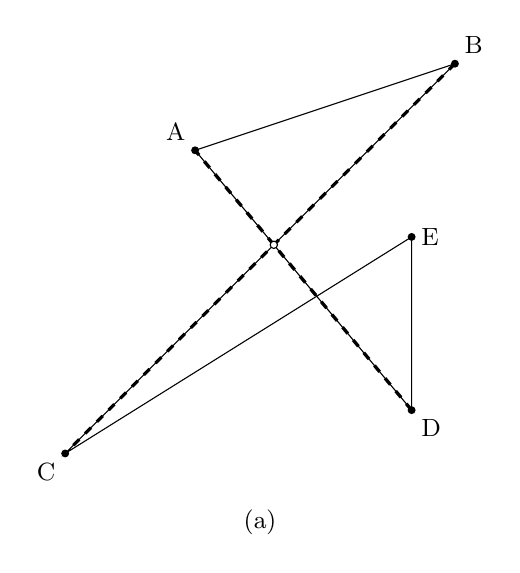
\begin{tikzpicture}[scale=0.55,every node/.style={font=\small}]
  \draw (8,5) -- (8,1) -- (3,7) -- (9,9) -- (0,0) -- (8,5);
  \draw[very thick,dashed] (8,1) -- (3,7);
  \draw[very thick,dashed] (9,9) -- (0,0);
  \filldraw[fill=white,draw=black] (4.818,4.818) circle (2.4pt);
  \fill (3,7) circle (2.6pt) node[above left] {A};
  \fill (9,9) circle (2.6pt) node[above right] {B};
  \fill (0,0) circle (2.6pt) node[below left] {C};
  \fill (8,1) circle (2.6pt) node[below right] {D};
  \fill (8,5) circle (2.6pt) node[right] {E};
  \node at (4.5,-1.6) {(a)};
\end{tikzpicture}
\end{minipage}\hfill
\begin{minipage}{0.48\textwidth}
\centering
\begin{tikzpicture}[scale=0.55,every node/.style={font=\small}]
  \draw (8,5) -- (8,1) -- (0,0) -- (3,7) -- (9,9) -- (8,5);
  \fill (3,7) circle (2.6pt) node[above left] {A};
  \fill (9,9) circle (2.6pt) node[above right] {B};
  \fill (0,0) circle (2.6pt) node[below left] {C};
  \fill (8,1) circle (2.6pt) node[below right] {D};
  \fill (8,5) circle (2.6pt) node[right] {E};
  \node at (4.5,-1.6) {(b)};
\end{tikzpicture}
\end{minipage}
\caption{Instância de cinco cidades. (a) Rota inicial obtida pelo vizinho mais próximo; as arestas tracejadas $D$--$A$ e $B$--$C$ se cruzam. (b) Rota final após as duas trocas 2-opt da Subseção 2.4.3, sem cruzamentos.}
\label{fig:rotas-2opt}
\footnotesize{\textit{Fonte:} Elaborado pelos autores (2026)}.
\end{figure}

\subsection{Primeira iteração}

A primeira iteração avalia todos os pares de arestas não adjacentes da rota inicial. A Tabela~\ref{tab:candidatos-2opt} resume os cinco movimentos possíveis. O maior ganho remove $D$--$A$ e $B$--$C$ e insere $D$--$B$ e $A$--$C$:
\begin{equation}
    \Delta = 8{,}06 + 7{,}62 - 7{,}81 - 12{,}73 = -4{,}86,
    \label{eq:primeira-troca}
\end{equation}
produzindo a rota $E \rightarrow D \rightarrow B \rightarrow A \rightarrow C \rightarrow E$, com custo $35{,}44$ km. O movimento elimina o cruzamento e substitui duas arestas longas por duas mais curtas.

\begin{table}[htb]
\centering
\caption{Movimentos 2-opt avaliados na primeira iteração. Em negrito, o de maior ganho.}
\label{tab:candidatos-2opt}
\small
\renewcommand{\arraystretch}{1.2}
\begin{tabular}{|>{\raggedright\arraybackslash}p{4.6cm}|>{\raggedright\arraybackslash}p{4.2cm}|>{\raggedright\arraybackslash}p{1.3cm}|>{\raggedright\arraybackslash}p{2.1cm}|}
\hline
\rowcolor{gray!20}
\textbf{Arestas removidas} & \textbf{Arestas inseridas} & \textbf{$\Delta$} & \textbf{Custo resultante} \\ \hline
\textbf{$D$--$A$ ($7{,}81$) e $B$--$C$ ($12{,}73$)} & \textbf{$D$--$B$ ($8{,}06$) e $A$--$C$ ($7{,}62$)} & \textbf{$-4{,}86$} & \textbf{$35{,}44$} \\ \hline
$E$--$D$ ($4{,}00$) e $B$--$C$ ($12{,}73$) & $E$--$B$ ($4{,}12$) e $D$--$C$ ($8{,}06$) & $-4{,}54$ & $35{,}75$ \\ \hline
$A$--$B$ ($6{,}32$) e $C$--$E$ ($9{,}43$) & $A$--$C$ ($7{,}62$) e $B$--$E$ ($4{,}12$) & $-4{,}02$ & $36{,}28$ \\ \hline
$D$--$A$ ($7{,}81$) e $C$--$E$ ($9{,}43$) & $D$--$C$ ($8{,}06$) e $A$--$E$ ($5{,}39$) & $-3{,}80$ & $36{,}50$ \\ \hline
$E$--$D$ ($4{,}00$) e $A$--$B$ ($6{,}32$) & $E$--$A$ ($5{,}39$) e $D$--$B$ ($8{,}06$) & $+3{,}12$ & $43{,}42$ \\ \hline
\end{tabular}

\footnotesize{\textit{Fonte:} Elaborado pelos autores (2026)}
\end{table}

Os demais movimentos também reduzem o custo, mas em menor grau; o último aumenta o custo e é rejeitado. A escolha do maior ganho é a regra da melhor melhoria. Observe que o movimento de maior ganho é justamente o que remove o cruzamento, o que confirma a intuição geométrica discutida na seção anterior.

\subsection{Segunda iteração e critério de parada}

A segunda iteração parte da rota $E \rightarrow D \rightarrow B \rightarrow A \rightarrow C \rightarrow E$. O maior ganho remove $D$--$B$ e $C$--$E$ e insere $D$--$C$ e $B$--$E$:
\begin{equation}
    \Delta = 8{,}06 + 4{,}12 - 8{,}06 - 9{,}43 = -5{,}31,
    \label{eq:segunda-troca}
\end{equation}
chegando a $E \rightarrow D \rightarrow C \rightarrow A \rightarrow B \rightarrow E$, com custo $30{,}13$ km (Figura~\ref{fig:rotas-2opt}(b)). A rota já não apresenta cruzamentos; o ganho vem de encurtar a conexão $C$--$E$ e reorganizar o contorno da rota.

Na terceira iteração, todos os cinco movimentos 2-opt aumentam o custo (o menor $\Delta$ é $+3{,}12$), de modo que o algoritmo para. A solução encontrada é, portanto, 2-ótima: nenhuma troca de duas arestas a melhora. Fixando a cidade $E$ e permutando as quatro demais, obtêm-se $4!/2 = 12$ ciclos distintos; enumerando-os, o menor custo é $30{,}13$ km, obtido pelo ciclo $A \rightarrow B \rightarrow E \rightarrow D \rightarrow C \rightarrow A$, que é o mesmo ciclo $E \rightarrow D \rightarrow C \rightarrow A \rightarrow B \rightarrow E$ percorrido no sentido oposto. Nesta instância, portanto, o 2-opt alcançou o ótimo global.

\section{Comparação entre a Solução Inicial e a Solução Após a Tentativa de Melhoria}

A Tabela~\ref{tab:comparacao-2opt} compara as soluções. A rota inicial, com $40{,}30$ km, é reduzida para $35{,}44$ km após a primeira troca (redução de $12{,}06\%$) e para $30{,}13$ km após a segunda (redução de $25{,}24\%$). A rota final coincide com a ótima e não possui cruzamentos.

\begin{table}[htb]
\centering
\caption{Comparação entre a solução inicial, as soluções obtidas pelo 2-opt e a solução ótima.}
\label{tab:comparacao-2opt}
\small
\renewcommand{\arraystretch}{1.25}
\begin{tabular}{|>{\raggedright\arraybackslash}p{4.4cm}|>{\raggedright\arraybackslash}p{3.6cm}|c|>{\raggedright\arraybackslash}p{3.2cm}|}
\hline
\rowcolor{gray!20}
\textbf{Solução} & \textbf{Rota} & \textbf{Custo (km)} & \textbf{Redução em relação à inicial} \\ \hline
Inicial (vizinho mais próximo) & $E$--$D$--$A$--$B$--$C$--$E$ & $40{,}30$ & --- \\ \hline
Após a primeira troca & $E$--$D$--$B$--$A$--$C$--$E$ & $35{,}44$ & $12{,}06\%$ \\ \hline
Após a segunda troca (final) & $E$--$D$--$C$--$A$--$B$--$E$ & $30{,}13$ & $25{,}24\%$ \\ \hline
Ótima (enumeração completa) & $A$--$B$--$E$--$D$--$C$--$A$ & $30{,}13$ & $25{,}24\%$ \\ \hline
\end{tabular}

\footnotesize{\textit{Fonte:} Elaborado pelos autores (2026)}
\end{table}

O primeiro movimento é o de maior ganho porque remove o cruzamento e substitui duas arestas longas por duas mais curtas. O segundo não remove cruzamento algum, mas encurta a conexão $C$--$E$, que era longa na rota intermediária. A soma dos dois ganhos explica a redução de $25{,}24\%$ em relação à solução gulosa. A busca local, portanto, corrigiu uma decisão local ruim do vizinho mais próximo sem reconstruir a rota desde o início \cite{johnson1997}.

A rota final é 2-ótima, pois todos os cinco movimentos 2-opt aumentam o custo. Nesta instância, a enumeração completa confirma que ela também é globalmente ótima. Esse resultado, porém, é uma coincidência favorável: em outras instâncias, a busca local pode parar em um ótimo local cujo custo é significativamente maior que o ótimo global, como discutido na seção seguinte.

\section{Limitações das Estratégias de Busca Local}

A principal limitação da busca local é que ela garante apenas otimalidade local. Uma rota 2-ótima pode exigir a remoção simultânea de três ou mais arestas para melhorar, possibilidade que nenhum movimento 2-opt isolado revela. Papadimitriou e Steiglitz \cite{papadimitriou1977} mostraram que, a menos que $P = NP$, nenhum algoritmo de busca local com tempo polinomial por iteração garante razão de aproximação constante para o TSP: existem instâncias em que o ótimo local está arbitrariamente longe do global. Assim, o fato de o algoritmo parar não significa que a rota seja boa em relação ao ótimo.

O resultado também depende da solução inicial e da vizinhança. Pontos de partida diferentes levam a bacias de atração diferentes, e uma vizinhança pequena pode não conter o movimento necessário para sair de um ótimo local. Práticas como multi-start, perturbação por double bridge (busca local iterada), simulated annealing e tabu search amenizam o problema, mas não eliminam a ausência de garantia. Além disso, a escolha de parâmetros e a ordem de avaliação dos movimentos influenciam o tempo de execução e a qualidade final \cite{souza_ufop, goldbarg2005, aarts2003}.

O custo por iteração do 2-opt é $O(n^2)$, mas o número de iterações pode ser exponencial no pior caso. Englert, Röglin e Vöcking \cite{englert2014} analisaram o 2-opt e mostraram que, embora o algoritmo seja rápido em muitos casos, existem instâncias em que ele realiza um número muito grande de iterações. Na prática, porém, o método converge rapidamente e fica a poucos pontos percentuais do ótimo em instâncias euclidianas, especialmente quando combinado com vizinhanças maiores e estruturas de dados eficientes \cite{johnson1997, helsgaun2000}.

\begin{table}[htb]
\centering
\caption{Limitações da busca local e possíveis mitigações.}
\label{tab:limitacoes-busca-local}
\small
\renewcommand{\arraystretch}{1.25}
\begin{tabular}{|>{\raggedright\arraybackslash}p{3.8cm}|>{\raggedright\arraybackslash}p{5.2cm}|>{\raggedright\arraybackslash}p{4.2cm}|}
\hline
\rowcolor{gray!20}
\textbf{Limitação} & \textbf{Consequência} & \textbf{Mitigação} \\ \hline
Ótimo local & A solução pode ser a melhor da vizinhança e estar longe do ótimo global. & Vizinhanças maiores, 3-opt, Lin--Kernighan e perturbações. \\ \hline
Dependência da solução inicial & Pontos de partida diferentes produzem resultados diferentes. & Multi-start e construções diversificadas. \\ \hline
Custo computacional & $O(n^2)$ por iteração no 2-opt e número de iterações não polinomial no pior caso. & Estruturas de dados eficientes, listas de vizinhos e critérios de parada. \\ \hline
Ausência de certificado & Parar não prova que a rota é globalmente ótima. & Limites inferiores e métodos exatos (branch-and-bound). \\ \hline
\end{tabular}

\footnotesize{\textit{Fonte:} Elaborado pelos autores (2026)}
\end{table}

Por fim, ao parar, o algoritmo certifica apenas que não há melhoria na vizinhança; ele não fornece um certificado de otimalidade global. Para provar que uma rota é ótima, são necessários limites inferiores ou métodos exatos, como o backtracking e o branch-and-bound discutidos nos próximos capítulos. A busca local, portanto, é uma ferramenta eficiente para melhorar rapidamente uma solução viável, mas não substitui os métodos que garantem otimalidade \cite{cormen2012, miyazawa_intro}.
